\documentclass{beamer}

\usepackage[frenchb]{babel}
\usepackage[utf8]{inputenc}  
\usepackage[T1]{fontenc}
\usepackage[lined,ruled,boxed,linesnumbered]{algorithm2e}
\usepackage{amsmath,amsfonts,amsbsy,amssymb,mathabx,amsthm,bbm,bm} 
\usepackage{graphicx}
\usepackage{arydshln}
\usepackage{stmaryrd}

\usetheme{Warsaw}

\title{Codes LDPC}
\author{Banier Corentin et Karboul Maher}
\institute{Université de Bordeaux}
\date{18 Mai 2021}

\begin{document}
	\begin{frame}
        \titlepage
	\end{frame}

    \begin{frame}
        \frametitle{Introduction et présentation des objectifs}
        Dans ce travail, nous allons étudier, dans un premier temps, comment fabriquer des instances de code LDPC notamment avec le modèle Gallager. Puis, nous comprendrons comment décoder ces codes en effectuant un tas d'expériences. Et à la fin de ce projet, on essaiera d'optimiser ce dernier en limitant le nombre d'équations à satisfaire par un mot de code erroné.
    \end{frame}

    \begin{frame}
        \frametitle{Définition d'un code LDPC}
        \textsc{\textbf{\underline{Définition :}}} Un code LDPC régulier est défini comme l'espace nul d'une matrice de contrôle de parité $H$, qui a les propriétés suivantes:
        \begin{enumerate}
            \item Chaque ligne à $p$ valeurs 1.
            \item Chaque colonne à $q$ valeurs 1.
            \item $p$ et $q$ ont des valeurs petites en comparaison avec la longueur du code et avec le nombre de lignes de la matrice $H$.
        \end{enumerate}
    \end{frame}

    \begin{frame}
        \frametitle{Réprésentation des codes LDPC}
        Les codes LDPC peuvent être représentés sous forme matricielle ou sous la forme d'un graphe biparti.
        \newline Par exemple, la matrice suivante:
        $$H=
        \begin{pmatrix}
            1 & 0 & 0 & 0 & 1 & 0 & 0 & 0 \\
            0 & 1 & 0 & 0 & 1 & 1 & 0 & 0 \\
            0 & 0 & 1 & 0 & 0 & 1 & 1 & 0 \\
            0 & 0 & 0 & 1 & 0 & 0 & 1 & 1 
        \end{pmatrix}
        \quad
        $$
        Peut être définie de la manière suivante:
        \begin{figure}[!h]
            \centering
            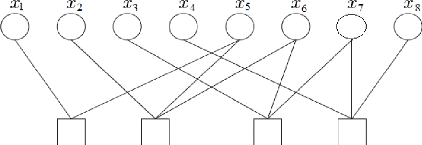
\includegraphics[scale=0.5]{Tanner2.png}  
            \caption{Graphe de Tanner associé à $H$}
            \label{fig:Tanner2}
        \end{figure}
    \end{frame}

    \begin{frame}
        \frametitle{Construction des codes LDPC}
        \framesubtitle{Robert Gray Gallager}
        \begin{columns}
            \begin{column}{5cm}
                \begin{figure}[!h]
                    \centering
                    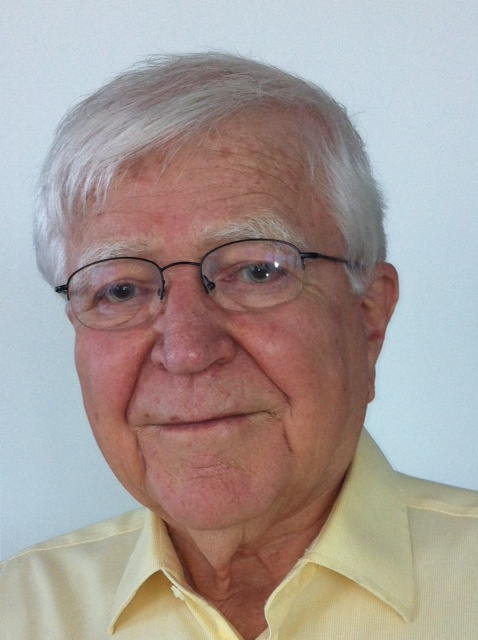
\includegraphics[scale=0.2]{Robert_Gallager.jpg} 
                    \caption{Mr. Robert Gray Gallager} 
                    \label{fig:gallager}
                \end{figure}
                Ingénieur Américain né en 1963.
            \end{column}
            
            \begin{column}{5cm}
                \begin{itemize}
                    \item Travaux sur le théorie de l'information.
                    \item Publication en 1963 de sa thèse sur les codes de contrôle de parité de basse densité (LDPC).
                    \item Rédacteur en chef adjoint sur le codage au sein de l’IEEE Transactions on Information Theory de 1963 à 1964.
                    \item Rédacteur associé pour les communications informatiques de 1977 à 1980.
                \end{itemize}
            \end{column}
            \end{columns}
    \end{frame}

    \begin{frame}
        \frametitle{Construction des codes LDPC}
        \framesubtitle{La construction de Gallager}
        On définit les $H_{i}$, les colonnes d'une matrice $H$.\newline
        Puis les $L_{j}$, les lignes d'une matrice $H$.\newline
        Et on note $\omega(x)$ le poids de $x$.\newline
        Voici un exemple d'une matrice de Gallager:
        $$H=
        \begin{bmatrix}
            1 & 1 & 1 & 1 & 1 & 0 & 0 & 0 & 0 & 0 \\
            0 & 0 & 0 & 0 & 0 & 1 & 1 & 1 & 1 & 1 \\
            \hdashline
            1 & 0 & 1 & 0 & 0 & 1 & 0 & 1 & 0 & 1 \\
            0 & 1 & 0 & 1 & 1 & 0 & 1 & 0 & 1 & 0 \\
            \hdashline
            1 & 1 & 0 & 0 & 1 & 0 & 1 & 0 & 0 & 1 \\
            0 & 0 & 1 & 1 & 0 & 1 & 0 & 1 & 1 & 0 
        \end{bmatrix}
        \quad
        $$
    \end{frame}

    \begin{frame}
        \frametitle{Construction des codes LDPC}
        \framesubtitle{Construction utilisée pour nos tests}
        DÉSINER UN EXEMPLE D'UNE MATRICE UTILISÉE
    \end{frame}

    \begin{frame}
        \frametitle{Algorithme de décodage}
        \begin{figure}[!h]
            \centering
            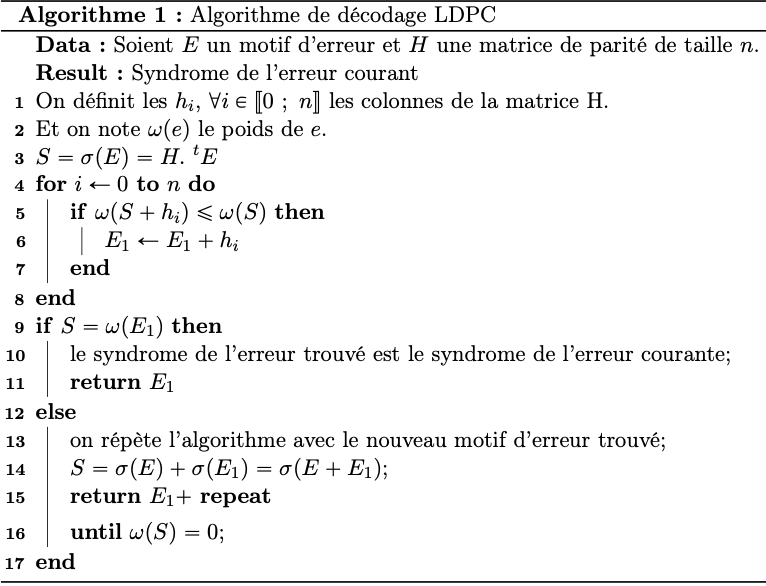
\includegraphics[scale=0.65]{algo.png}  
            \label{fig:algo}
        \end{figure}
    \end{frame}

    \begin{frame}
        \frametitle{Expérimentations}
    \end{frame}

    \begin{frame}
        \frametitle{Conclusion}
    \end{frame}

\end{document}